\documentclass[a4paper, 12pt]{article}
\usepackage[utf8]{inputenc}
\usepackage[russian]{babel}
\usepackage{literat}
\usepackage[T2A]{fontenc}
\usepackage{verse}
% \usepackage{geometry}
\usepackage[left=3cm, right=3cm, top=2cm, bottom=2cm]{geometry}
\usepackage[nottoc]{tocbibind}
% \usepackage[style=ieee]{biblatex}
\usepackage{biblatex}
\addbibresource{5_references.bib}
\usepackage{csquotes}
\usepackage{graphicx}
% \usepackage{setspace}

\graphicspath{ {./images/} }
\usepackage[export]{adjustbox}
\usepackage{hyperref}
\hypersetup{
    colorlinks,
    citecolor=black,
    filecolor=black,
    linkcolor=black,
    urlcolor=black
}
% \setlength\parindent{0pt}

% \title{доклад на тему\\\textbf{\scshape\Huge{Достижения арабских математиков в алгебре}}}
% \author{\Large{\scshapeАлександр Родионов}\\ФКН, МКН, 1к (магистратура)\\}


\begin{document}

% \maketitle

\thispagestyle{empty}

\begin{center}
ФЕДЕРАЛЬНОЕ ГОСУДАРСТВЕННОЕ БЮДЖЕТНОЕ ОБРАЗОВАТЕЛЬНОЕ УЧРЕЖДЕНИЕ ВЫСШЕГО ОБРАЗОВАНИЯ\\
<<ВОРОНЕЖСКИЙ ГОСУДАРСТВЕННЫЙ УНИВЕРСИТЕТ>>\\
\vspace{0.25cm}
Факультет компьютерных наук\\
\vspace{0.25cm}
Кафедра цифровых технологий\\

\vspace{1cm}

\textit{Математика и компьютерные науки}\\
\textit{Распределенные системы и искусственный интеллект}\\

\vspace{4cm}

\large{доклад на тему\\}
\Huge{\scshape{Достижения арабских математиков в алгебре}}

\vspace{3cm}


\begin{small}
\begin{tabbing}
ооооооооооооооо \=  ----------------------  \kill
Обучающийся \>  \rule[0mm]{3cm}{0,3mm}  \textit{А.А. Родионов, 1 курс, (магистратура)} \\ 
ооооооооооооооо \=  ----------------------  \kill
Преподаватель\>  \rule[0mm]{3cm}{0,3mm}  \textit{С.А. Скляднев, к. физ-мат. н., доцент }
\end{tabbing}

\vspace{9cm}

\centerline{Воронеж 2018}
\end{small}

\end{center}


% \newpage
\tableofcontents

\section{Введение}
Развитие арабской математики началось в 7 в. нашей эры, как раз  в эпоху возникновения религии  ислама. Она выросла из многочисленных  задач, поставленных торговлей, архитектурой, астрономией, географией, оптикой, и глубоко сочетала  в себе стремление решить эти практические задачи и напряженную  теоретическую работу.

Арабские  математики добились решающих  достижений и сделали ряд неоспоримых   открытий в области разработки  алгебраического исчисления, как  абстрактного, так и практического,  становления теории уравнений, алгоритмических методов на стыке алгебры и арифметики.

В развитии арабской математики  можно  различить два периода:  прежде всего  усвоение в  VII и VIII вв. греческого и восточного  наследия. Багдад был первым крупным  научным центром в правления Аль-Мансура (754-775) и Гарун ал-Рашида (786-809). Там было большое количество  библиотек, и изготовлялось много  копий научных трудов. Переводились  труды античной Греции (Евклид, Архимед,  Аполлоний, Герон, Птолемей, Диофант), изучались также труды из Индии, Персии и Месопотамии. 

Но  к IX в. сформировалась настоящая  собственная математическая культура, и новые работы вышли за  рамки, определенные эллинским  математическим наследием.

Первым  знаменитым ученым багдадской  школы был Мухаммед Аль-Хорезми, деятельность которого протекала в первой половине IX в. Он входил в группу математиков и астрономов, которые работали в Доме мудрости, своего рода академии, основанной в Багдаде в правление ал-Маммуна (813-833). Сохранились пять работ ал-Хорезми, частично переработанные, из которых два трактата об арифметике и алгебре оказали решающее воздействие на дальнейшее развитие математики.

Его  трактат об арифметике известен  только в латинском варианте XIII в., который, без сомнения, не является  точным переводом. Его можно  было бы озаглавить «Книга  о сложении и вычитании на  основе индийского исчисления».  Это, во всяком случае, первая  книга, в которой изложены десятичная  система счисления и операции, выполняемые в этой системе,  включая умножение и деление.  В частности, там использовался  маленький кружочек, выполнявший  функции нуля. Ал-Хорезми объяснял, как произносить числа, используя понятия единицы, десятка, сотни, тысячи, тысячи тысяч…, которые он определил. Но форма использованных ал-Хорезми цифр неизвестна, возможно, это были арабские буквы или арабские цифры Востока.
 
О  происхождении  арабских цифр  стоит сказать отдельно.   Арабские  цифры — традиционное название  десяти математических знаков: 0, 1, 2, 3, 4, 5, 6, 7, 8, 9, с помощью которых  по десятичной системе счисления  записываются любые числа. Эти  цифры возникли в Индии (не  позднее V в.), в Европе стали  известны в Х-ХIII вв. по арабским сочинениям (отсюда название).  

Интересные  факты: Ряд интересных математических задач, стимулировавших развитие сферической геометрии и астрономии, поставила перед математикой и сама религия ислама. Это задача о расчёте лунного календаря, об определении точного времени для совершения намаза, а также об определении киблы — точного направления на Мекку.  

\section{Аль-Хорезми}
\subsection{Биография}
Начнем с обсуждения аль-Хорезми, отца алгебры. Абу Абдулла Мухаммад ибн Муса Аль-Хорезми жил около 800-847 н.э., но эти даты неточны. Эпитет «аль-Хорезми» относится к его месту происхождения, Хорезму или Хорезму, который расположен к югу от дельты реки Аму-Дарья и Аральского моря в Центральной Азии. Однако историк аль-Табари добавляет эпитет «аль-Кутруббулли», указывая, что аль-Хорезми в действительности прибыл из Кутрубулла, недалеко от Багдада между реками Тигр и Евфрат. Другие источники утверждают, что, возможно, предки аль-Хорезми, а не он сам, происходят из Хорезма. Еще одним интересным эпитетом, добавленным аль-Табари, является «аль-Маюси», что означало бы, что аль-Хорезми был приверженцем Зороастрийская религия. Однако предисловие аль-Хорезми к его трактату о альберте не вызывает сомнений, что он был набожным мусульманином; возможно, некоторые из его предков или даже аль-Хорезми в юности были зороастрийцами.

Аль-Хорезми вырос под Багдадом под властью Калифа аль-Мамуна (царствование 813-833 гг. Н.э.), который был великим пропагандистом науки. Аль-Хорезми была предложена должность в Байт-аль-Хикме (Дом Мудрости) в Багдаде; большинство его трактатов посвящено халифу аль-Мамуну.

\subsection{Математический вклад Аль-Хорезми}
\subsubsection{Астрономия}
Большинство трактатов аль-Хорезми относятся к области астрономии. Он был одним из разработчиков астролябии, а также составил примерно сотню астрономических таблиц. Одна из этих таблиц, Зидж Аль-Синдхинд (перевод индийской работы, Зидж — общее название для астрономических таблиц в странах ислама.), является первой арабской астрономической работой из всех которые сохранились. 

\subsubsection{География}
Он также написал текст географии, Китаб сурат аль-ард, в котором перечислены долготы и широты городов и населенных пунктов. Это было основано на карте мира аль-Мамуна, на которой работал аль-Хорезми, которая, в свою очередь, была основана на географии Птолемея. Однако карта мира аль-Мамуна была гораздо более точной, чем Птолемея, особенно в отношении исламского мира.

\subsubsection{Календарь}
Еще одна сохранившаяся работа аль-Хорезми - это его работа над еврейским календарем, в котором точно описывается 19-летний цикл, семь месяцев и правила определения, в какой день недели начинается месяц Тишри. Он также подсчитывает интервал между еврейской эрой или созданием Адама и эры Селуддида, которая началась 1 октября 312 года до нашей эры. Также, аль-Хорезми включает метод определения средней долготы Солнца и Луны.


\subsubsection{Арифметика}
В дополнение к его работам по алгебре, трактаты аль-Хорезми, которые обеспечили его прочную славу, - его работы по арифметике. Его арифметический трактат, возможно, озаглавлен «Китаб аль-иам ва'л-тафрик би-абаб аль-Хинд», или «Книга добавления и вычитания» по методу расчета индусов. Однако оригинальная арабская рукопись теперь потеряна, и его текст сохранился только в ее латинском переводе, который, возможно, сделал Аделард из Бата в 12 веке. Впервые он был опубликован в 1857 году в журнале «Algoritmi de numero indorum» Б. Бонкомпаньи, а затем опубликован в 1963 году как «Алгоритм Мохаммеда ибн Муса Альхваризми» Курта Фогеля. Это первый известный учебник о десятичной системе, и это первый трактат который систематически излагает использование арабских (или иногда индусско-арабских) цифр 1-9, 0 и позиционной системы счисления.\cite{mohamed} Ввод в использование числа 0 было самым важным; «маленький круг на самом деле является одной из величайших математических инноваций в мире».\cite{mohamed} Символ 0 использовался около 250 лет в исламском мире после его введения аль-Хорезм прежде чем западный мир когда-либо узнал об этом.

Современная цифровая нотация, безусловно, имеет свои корни в аль-Хорезми и других арабских математиках; хотя под влиянием индуистских цифр аль-Хорезми и его арабские преемники ввели полную концепцию десяти чисел и метод десятичных обозначений\cite{mohamed}. Аль-Хорезми представил ноль, и его способ счисления индийских цифр был настолько точными, что он, вероятно, был ответственен за распространенное мнение о том, что наша система счисления - арабская. Хотя аль-Хорезми никогда не претендовал на оригинальность в отношении своей системы чисел, латинские переводы его произведений были широко распространены в Европе, а неосторожные читатели приписывали автора и нумерацию автору\cite{boyer}. Именно эта связь с числами привело к искажению имени аль-Хорезми к алгоризму, что, в свою очередь, привело к современному слову алгоритм.

\subsection{Алгебра Аль-Хорезми}
\subsubsection{Аль-джабр и Аль-мукабала}
В интересах этой статьи наиболее важной темой будет трактат аль-Хорезмита \textit{Китаб аль-джабр ва'л-мукабала}, или \textit{Книга восстановления и балансировки} \cite{boyer}. Значения слов \textit{аль-джабр} и \textit{аль-мукабалах} обсуждаются. Аль-джабр, которое пришло к нам в форме «алгебры», вероятно, имелось в виду нечто вроде «восстановления» или «завершения», ссылающееся на перенос членов на другую сторону уравнения с отрицательным знаком или добавление одинаковых членов к обоим сторонам уравнения чтобы устранить отрицательные члены \cite{boyer}. Аль-мукабала, вероятно, означает нечто вроде «восстановления» или «балансировки», ссылаясь на вычеркивание подобных членов с противоположных сторон уравнения или уменьшение положительных членов на вычитание равных значений из обеих сторон уравнения\cite{boyer}, 257. Вместе два слова аль-джабр и аль-мукабала могут означать науку об алгебре. В трактате Аль-Хорезми была первая книга, в которой этот титул обозначался как отдельная дисциплина.

Может быть полезно увидеть примеры того, как аль-Хорезми использовали эти термины. Он сначала ставит проблему:

\begin{displayquote}
Я разделил десять на две части. Я умножил одну из двух частей на другую. После этого я умножил одну из частей саму на себя. Результат умножения само на себя в четыре раза больше, чем произведение одной из частей на другую.\cite{vanderwaer}
\end{displayquote}

Аль-Хорезми называет одну из частей «вещь», а другую «десять минус вещь. Он умножает на два, получает «десять вещей минус квадрат», а затем получает (в современных обозначениях):

$$x^2 = 40x - 4x^2$$

Он использует \textit{аль-джабр} для добавления $4x^2$ к обеим сторонам, что дает:

$$5x^2 = 40x$$

Аль-Хорезми затем получает

$$x^2 = 8x$$

из которого он получает

$$x = 8$$

(Для современного читателя очевидно, что аль-Хорезми не допускает $x$
равным $0$)

На другой странице у аль-Хорезми есть уравнение:

$$50 + x^2 = 29 + 10x$$

Он использует \textit{аль-мукабалах}, чтобы вычесть из обоих сторон $29$, чтобы получить:

$$21 + x^2 = 10x$$

\subsubsection{Происхождение алгебры}
Важно отметить, что \textit{Происхождение алгебры} уходит корнями к древним египтянам и вавилонянам, у которых были тексты, посвященные проблемам арифметики, алгебры и геометрии еще в 2000 году до нашей эры. В «Арифметике» Диофанта уже появилось несколько уравнений. Однако эти уравнения были решены как часть решений других проблем и не подвергались систематической обработке. Аль-Хорезми был первым, кто систематически изучал алгебру. Хотя существовали уравнения Диофанта, аль-Хорезми, вероятно, не знал о них в то время, когда писал свой трактат; аль-Хорезми не знал греческого языка, и в то время не было арабского перевода Арифметики. На Аль-Хорезми, вероятно, больше влияли индуистские или местные сирийско-персидско-еврейские источники. Однако ни один из этих источников не перешел к аль-Хорезми; несколько текстов, которые, по-видимому, были написаны после Китаб аль-Джабра ва'л-мукабала. Некоторые западные исследователи утверждают, что Аль-Хорезми не является «настоящим математиком», поскольку «в его работе мало того, чего нельзя найти в более ранних индийских источниках».

\subsubsection{Алгебраические уравнения}
\textit{Китаб аль-джаб ва'л-мукабала} состоит из трех секций, первая из которых утверждает, что все линейные и квадратичные уравнения могут быть сведены к одному из шести типов:

$$ax^2 = bx$$
$$ax^2 = b$$
$$ax = b$$
$$ax^2 + bx = c$$
$$ax^2 + c = bx$$
$$ax^2 = bx + c$$

Он представляет общие решения для всех этих типов. Рассматривая эти шесть уравнений, очевидно, что аль-Хорезми не принимал отрицательные или нулевые коэффициенты.

Трактаты Аль-Хорезми о смешанных квадратичных уравнениях («корни и числа, равны квадратам», «квадраты и числа, равны корням») лучше всего рассматривать на примере первого типа смешанных квадратичных уравнений. В словах аль-Хорезми:


\begin{displayquote}
\textit{Корни и квадраты, равны числам}
Например: один квадрат и десять корней одного и того же значения равны тридцати девяти дирхемов; то есть, какова должна быть площадь, которая, если ее увеличить на десять собственных корней, составляет тридцать девять?

Решение: вы сокращаете вдвое количество корней, которые в данном примере дают пять. Это вы умножаете само на себя; произведение составляет двадцать пять. Добавьте это к тридцати девяти; сумма составит шестьдесят четыре. Теперь возьмите корень этого, который равен восьми, и вычтите из него половину числа корней, что равно четырем. Отстаток три. Это корень площади, о которой вы думали; сам квадрат равен девяти.
\end{displayquote}

В современных обозначениях уравнение имеет вид:

$$x^2 + 10x = 39$$

и решение Аль-Хорезми это:

$$(x + 5)^2 = 39 + 25 = 64$$
$$x + 5 = \sqrt{64} = 8$$
$$x = 8 -5 = 3$$
$$x^2 = 9$$

Ал-Хорезми демонстрирует это решение с помощью квадрата $AB$, стороной которого является искомый корень x. На каждой из четырех сторон он строит прямоугольники, каждый из которых имеет ширину 2.5. Итак, квадрат вместе с четырьмя прямоугольниками равен 39. Чтобы заполнить квадрат $EH$, аль-Хорезми добавляет четыре раза квадрат 2.5 или 25. Таким образом, площадь большого квадрата $EH$ равна 64, а его сторона равна 8 Таким образом, сторона x исходного квадрата $AB$ равна $8 - 5 = 3$ (см. рисунок ниже).

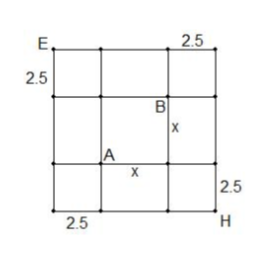
\includegraphics[scale=0.5, center]{1}

Аль-Хорезми также представляет более простой похожий метод, который строит прямоугольники ширины 5 с двух сторон квадрата $AB$. Тогда общая площадь квадрата $EH$ равна $x^2 + 10x + 25 = 39 + 25 = 64$, что дает тот же результат $x = 3$ или $x^2 = 9$ (см. рисунок ниже).

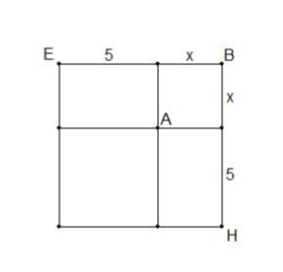
\includegraphics[scale=0.5, center]{2}

Аль-Хорезми также обсуждает методы извлечения квадратного корня; этот метод, возможно, был адаптирован из индуистских источников. Этоn метод проще всего объяснить на примере. Чтобы найти квадратный корень из 107584, «вертикальные линии нарисованы и цифры разбиты на периоды по две цифры». Ближайший корень из 10 равен 3, и поэтому его квадрат равный 9 вычитается из 10. 3 написанно ниже всего, как часть окончательного квадратного корня. 3 удваивается, чтобы сделать 6, что содержится дважды в 17; $6 \times 2 = 12$, поэтому 12 вычитается из 17 что оставляет 5. Таким образом, 2 записывается внизу как следующая часть окончательного квадратного корня. Затем квадрат 2 (который равен 4) вычитается из 55, что дает в остатке 51. Таким образом, 518 затем делится на двойное 32 (что равно 64), оставляя 8. Таким образом, $8 \times 64 = 512$ вычитается из 518 оставляя 6. Последняя цифра тогда равна 64, что составляет 8 в квадрате, поэтому последняя цифра конечного квадратного корня равна 8. Следовательно, квадратный корень из 107584 равен 328. (рисунок ниже).

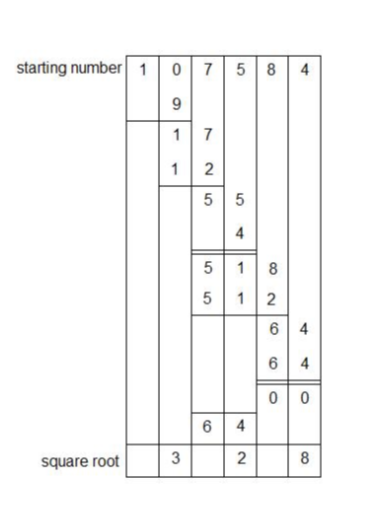
\includegraphics[scale=0.5, center]{3}

\subsubsection{Мероопределение}
Вторая глава \textit{Алгебры} Аль-Хорезми относится к вопросу о мерах. В нем изложены правила для вычисления площадей и объемов. Площадь круга можно найти, умножив половину диаметра на половину окружности. Чтобы найти окружность, аль-Хорезми предоставляет три правила.

С диаметром $d$ и окружностью $p$ и приблизительным значением $\pi = p / d$:

$$p = 3\frac{1}{7}d\textrm{, или } \pi \approx 3.1439$$
$$p = \sqrt{10d^2}d\textrm{, или } \pi \approx 3.1639$$
$$p = \frac{62832}{20000}d\textrm{, или } \pi \approx 3.1416$$

Первое правило было сформулировано Архимедом и также было дано в \textit{Метрике} Герона Александрийского и в еврейском трактате \textit{Мишнат ха-Миддот}. Второе приведенное правило можно найти в \textit{Брахмашфутасиддханте} Брахмагупты. Третий (эквивалентный точной оценке $\pi \approx 3.1416$) приписывается «Астрономам» Аль-Хорезми, который может относиться к индусскому астроному Ариабхате; то же правило можно найти в его «Арябхатии».

Аль-Хорезми также утверждает, что для прямоугольного треугольника со сторонами $a$, $b$ $c$, с «короткими» сторонами $a$ и $b$:

$$a^2 + b^2 = c^2$$

Он дает доказательство в тексте; однако его доказательство справедливо только для равностороннего треугольника, когда $a = b$. Из этого видно, что основной источник Аль-Хорезми не может быть классическим греческим трактатом, таким как \textit{Начала} Евклида. Еврейский трактат \textit{Мишнат ха-Миддот} тесно связан с главой Аль-Хорезми о измерениях, которая показывает какую-то прямую зависимость или общий источник обоих. Если Соломон Гандс прав, автор еврейского трактата был раввином Неемии, который жил около 150 г. н.э., Аль-Хорезми, возможно, полагался на трактат или на перевод или текст перевода в Перине или Сирии. Однако другие авторы быстро указывают на то, что вывод Соломона Гандса не подтвержден, что оставляет дату появления Мишнат ха-Миддо открытым даже до того периода, когда аль-Хорезми опубликовал свою Алгебру. Гад Сарфатти утверждает, что Мишнат ха-Миддот был написан не позднее позднего исламского периода и может быть адаптацией работы Аль-Хорезми.

\subsubsection{Наследия}
Последняя глава Алгебры является самой большой. Она целиком состоит из задач и решений, включающих простые арифметические и линейные уравнения. Эти проблемы не будут обсуждаться здесь, поскольку они используют ту же самую алгебру, которая уже обсуждалась.

\subsubsection{Влияние}
Алгебра Аль-Хорезми стала известна, как только она была опубликована, и мусульманские математики прокомментировали ее во время жизни Аль-Хорезми. Алгебра впервые стала известной на Западе, когда европейские ученые, такие как Аделард Бат (1120 г.) и Роберт Честер (1140 г.), начали переводить арабские произведения на латынь. Леонардо Пизанский, также известный как Фибоначчи, включает в себя многие задачи, связанные с Аль-Хорезми. Однако они, скорее всего, взяты из текстов Абу Камиля, в которых используются многие проблемы и решения Аль-Хорезми. Уильям Луна, еще один итальянский математик, перевел Алгебру Аль-Хорезми на итальянский язык в начале 13 века; на этот перевод ссылались несколько ученых в 16 веке. Влияние трактата Аль-Хорезми достигло работ Иоганнеса де Муриса в 14-м веке, Regiomontanus в 15 веке, а Адам Ризе, Перес де Мойя , Кардана и Адриан Ромена в 16 веке. Даже сегодня некоторые учителя элементарной алгебры используют предложения, уравнения и геометрические представления Аль-Хорезми, даже не зная их источника. Мохини Мохамед очень хорошо подытоживает прочное влияние аль-Хорезми, и поэтому я оставляю ее заключение:

\begin{displayquote}
Во момент его смерти наследие, которое Аль-Хорезми оставил в исламском сообществе, включало способ представления чисел, который привел к удобному методу вычисления, даже с дробями; наука об алгебре; и карту мира, которая является более точной, чем когда-либо прежде.

В западном мире математическая наука была более подвержена влиянию аль-Хорезми, чем любой другой средневековый писатель. Именно благодаря Аль-Хорезми мы можем широко использовать арабские цифры. Позиционная система счисления по основанию 10, свободное использование иррациональных чисел и его введение алгебры в современном смысле сделали его главной фигурой в истории мусульманской математики. Его введение арабских цифр изменило содержание и характер математики и произвело революцию в обычной практике расчета в Средневековой Европе. С интеграцией греческой, индуистской и, возможно, вавилонской математики в его алгебре этот текст является одним из лучших представлений международного символа исламской средневековой цивилизации. Среди прочего, слова алгебра, алгоритм, шифр и корень выжили в качестве свидетелей роли Аль-Хорезми в создании и распространении науки вычислений.
\end{displayquote}





\section{Дальнейшее развитие алгебры}
После инновационной Алгебры Аль-Хорезми, развитие алгебры не остановилось. Несколько мусульманских математиков известны своми работами в области алгебры.

\subsection{Сабит ибн Курра}
Сабит ибн Курра (836-901 н.э.) продолжил общие решения Аль-Хорезми; однако Аль-Хорезми представляет свои общие доказательства в
соединение с конкретными уравнениями, тогда как ибн Курра представляет свои решения обобщенно. В свое время ибн Курра имел полный доступ к Началам Евклида и свободно использовал теоремы Евклида в своих алгебраических доказательствах. 

В случае $x^2 + px = q$, Сабит ибн Курра верно находит, что $x = \sqrt{q + (\frac{p}{2})^2} - (\frac{p}{2})$. Он приводит общие доказательства, следуя примерам <<определение - теорема - доказательство>> Евклида.

\subsection{Абу Камил}
Абу Камил (около 850-930 н.э.) написал трактат под названием «Алгебра», который был комментарием к работе Аль-Хорезми. Его примеры позже были использованы как мусульманским ученым Аль-Караджи в конце 10 века, так и итальянским Леонардо Пизанским или Фибоначчи в конце 12 века. Многие из его примеров взяты из Аль-Хорезми. Абу Камиль также рассматривает геометрические доказательства решений уравнений в терминах конкретных примеров, как Аль-Хорезми, вместо использования общих доказательств, таких как Сабит ибн Курра. Абу Камиль выходит за пределы алгебры Аль-Хорезми и Сабит ибн Курра, предоставляя правила манипулирования следующими алгебраическими величинами:

$$(a \pm b)(b \pm qx) = ab \pm bpx \pm aqx + pqx^2$$
$$(a \pm b)(b \mp qx) = ab \pm bpx \mp aqx - pqx^2$$
$$\sqrt{ab} = \sqrt{a}\sqrt{b}$$
$$\sqrt{a/b} = \sqrt{a}/\sqrt{b}$$
$$\sqrt{a} \pm \sqrt{b} = \sqrt{a + b \pm 2\sqrt{ab}}$$

Абу Камиль дает как алгебраические, так и геометрические доказательства для этих уравнений.

\subsection{Абу Бакр Аль-Караджи}
Аль-Караджи (953-1029 н.э.) имеет тенденцию применять арифметику к алгебре, в отличие от Абу Камиля и Ибн Курры, которые применяют геометрию к алгебре. Абу Бакр Аль-Караджи написал \textit{Дивный}, в котором он развивает алгебру выражений с использованием высших степеней неизвестного. Он использует «корень», «сторону» или «вещь» для обозначения x, «mal» для x2, «куб» для x3, «mal mal» для x4, «mal куб» для x5 и т. д. Он создает каждую степень неизвестного путем умножения на предыдущие элементы; это новшество позволило аль-Караджи обращаться с такими уравнениями, как $x^4 + 4x^3 - 6$ и $5x^6 - (2x^2 + 3)$

\subsection{Аль Самуил (Самуил Марокканский)}
Ибн Яхья Аль-Магриби Аль-Самуил (1130-1180 гг. Н. Э.) Родился в Багдаде. Хотя он родился в еврейской семье, он обратился в ислам в 1163 году, когда ему приснился сон, говорящий ему об этом. Он был известным врачом и путешествовал по современному Ирану, чтобы заботиться о своих пациентах, в том числе о принцах. Его «Сияющая книга расчетов» дает правила для знаков, создавая понятия положительных (избыточных) и отрицательных (дефицитных) чисел. Затем он дает правила вычитания степеней:

$$(-ax^n) - (-bx^n) = -(ax^n - bx^n) \textrm{ ,если } a > b$$
$$(-ax^n) - (-bx^n) = +(bx^n - ax^n) \textrm{ ,если } a < b$$

Аль-Самуил излагает диаграмму, чтобы научить читателя, как умножать и делить
простые выражения, такие как «часть mal куба» или «mal mal куб, который
равны $\frac{1}{x^5}$ и $x^7$

Он также приводит примеры деления сложных многочленов, что было большим развитием в алгебре. Его первый пример показывает, как решить:

$$\frac{20x^6 + 2x^5 +58x^4 + 75x^3 + 125x^2 + 96x + 94 + 140x^-1 + 50x^-2 + 90x^-3 + 20x^-4}{2x^3 + 5x + 5 + 10x^-1}$$

Он создает диаграмму (рисунок ниже) с верхней строкой как имена порядков в естественной последовательности слева направо, а строка ниже - как строка ответа, которая начинается пустой и заполняется по мере продолжения. Остальная часть диаграммы разделена на горизонтальные полосы с двумя рядами каждая:

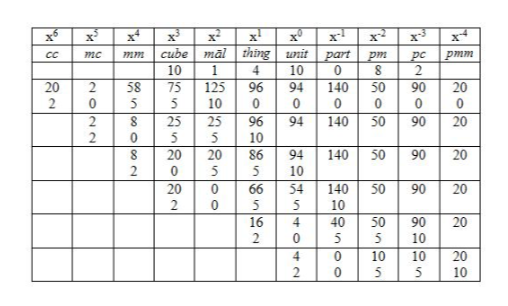
\includegraphics[scale=0.7, center]{4}

Аль-Самуил начинает с деления $20cc$ на $2c$ для получения $10c$, а затем вычитает ($10c \times$ делитель) из делимого. Старое делимое заменяется остатком после вычитания, а делитель копируется вправо. Повторяя эту процедуру, 2 нового делимого делится на 2 делителя, а частное 1 помещается в столбец справа от 10 в строке ответа. Аль-Самуил продолжает повторять процедуру до тех пор, пока не достигнет своего конечного результата:

$$10x^3 + x^2 + 4x + 10 + 8x^-2 +2x^-3$$

Аль-Самуил следует этому примеру с несколькими другими, повторяя ту же процедуру, но допуская отрицательные коэффициенты. Его открытие процедуры деления в столбик было значительным достижением в исламской алгебре.

\subsection{Омар Хайям}
Полное имя Омара Хайяма - Абу аль-Фат Омар бен Ибрагим Аль-Хайям и родился в современном Иране. Дословный перевод его имени означает «делатель палаток». Это, возможно было дело его отца. Хайям стал известен в результате популярного перевода Эдварда Фитцджеральда в 1859 году почти 600 коротких четырех стихотворений - Рубайята.

Его блестящий вклад был продолжен в XIX веке. Среди многих других он работал над вопросами, связанными c постулатом о параллельным прямых (пятый постулат Евклида). Используя четырехугольник, он обнаружил подход к исследованию, став стандартным. Он точно обнаружил, что нужно показать, чтобы доказать постулат о параллельных прямых, и именно на этих идеях была обнаружена неевклидова геометрия. Хайям также утверждал, что рациональные числа должны охватываться цифрами, отступающими от греческой традиции, влияние которых было тогда и должно было оставаться мощной силой в математике и философии до XIX века.

Он также обнаружил методы извлечения корня в сколь угодно большой степени. Он обнаружил (в алгебре) геометрический метод решения кубических уравнений путем пересечения параболы с кругом, но, по крайней мере частично, эти методы были описаны более ранними авторами, такими как Абу аль-Джуд. Чтобы увидеть, рассмотрим круг и параболу:

$$(x - a)^2 + y^2 = a^2 + c^2, y = x^2 + bx + c$$

Заменим и упросим:
$$x(x^3 - 2bx^2 -x -2cx -xb^2 +2a -2cb)$$

Что даст при делении:
$$x(x^3 + 2bx^2 +(1 + 2c + b^2)x + 2cb - 2a) = 0$$

Итак, пересечение x является решением кубического уравнения:

$$x^3 + 2bx^2 + (1 + 2c + b^2)x + 2cb - 2a$$
Хайям был выдающимся математиком и астрономом. Его работа над алгеброй была известна во всей Европе в средние века, и он также внес вклад в календарную реформу. Хайям упоминает в своей книге Алгебры другую работу, которая теперь потеряна. В этой потерянной работе Хайям обсуждает треугольник Паскаля, но китайцы, возможно, обсуждали треугольник перед этой датой.

Алгебра Хайяма является геометрической, решая линейные и квадратичные уравнения методами, появляющимися в Началах Евклида.

Известность Хайяма как поэта заставила некоторых забыть о его научных достижениях, которые были гораздо более существенными. Версии форм и стихов, используемых в Рубайяте, существовали в персидской литературе до Хайяма, и немногие из его стихов можно было отнести к нему с уверенностью.

\section{Источники арабской математики}
Важно взглянуть на используемые источники Аль-Хорезми, чтобы определить влияние греческой математики на его алгебру. Также важно обсудить современные источники Аль-Хорезми, или как современные ученые знают о работах Аль-Хорезми.

\subsection{Источники Аль-Хорезми}
Естественно начать с изучения источников, используемых Аль-Хорезми. Существует три теории, посвященные источникам, используемым Аль-Хорезми в начале алгебры; к ним относятся теории, в которых он использовал классические греческие источники, индуистские источники, популярные сирийско-персидско-ивритские математические труды

Согласно Тумеру, как описано в История альгебры Ван дер Вардена: от Fль-Хорезми до Эмми Нётер\cite{vanderwaer}, как индуистская, так и греческая алгебра вышли далеко за рамки элементарной стадии работы Аль-Хорезми. Доказательства, включенные в его работу, не имеют существенных различий в известных произведениях любой культуры. Например, его доказательства методов решения квадратичных уравнений существенно отличаются от доказательств, найденных в Элементах Евклида. Кроме того, сохранившийся алгебраический трактат греческой культуры, написанный Диофантом, развился в направлении символьного представления, в то время как  трактат Аль-Хорезми - риторический. В этом отношении работа ль-Хорезми аналогична работе санскритских алгебраических произведений. По этим причинам маловероятно, что на Аль-Хорезми значительно  повлияла классическая греческая математика.

Аль-Хорезми написал трактат об индусских цифрах, и двое из его приближений числа $\pi$ были найдены в индуистских источниках, поддерживая теорию о том, что на работу Аль-Хоризмами влияли индуистские источники. Аль-Хорезми далее ссылался на свои источники в своем разделе «Мероопределение / Мензурация» в своей Алгебре:

\begin{displayquote}
Однако у математиков есть два других правила. Одно из них: умножить диаметр на себя, затем на десять, а затем взять квадратный корень произведения. Корень дает длину окружности.

Другое правило используется среди астрономов и гласит: умножьте диаметр на шестьдесят две тысячи восемьсот тридцать два, а затем разделите его на двадцать тысяч. Частное дает длину окружности.
\end{displayquote}

Первое правило ($p = \sqrt{10d^2}d$) найдено в главе 12 \textit{Брахмашфутасиддханта} Брахмагупты, поддерживая теорию о том, что Аль-Хорезми был знаком с индуистскими алгебраическими трактатами. Аль-Хорезми
приписал второе правило ($p = \frac{62832}{20000}d$) к астрономам, и уравнение найдено в \textit{Aryabhatiya} индуистского астронома \textit{Aryabhata} с начала шестого века нашей эры. Поскольку Аль-Хорезми использовал как персидский, так и индуистский источники для составления своих астрономических таблиц, вполне вероятно, что он также получил свои оценки $\pi$ из этих источников.

Третья теория утверждает, что на работы Аль-Хорезми повлияла местная сирийско-персидско-ивритская традиция. Это подтверждается тесной связью между геометрией Аль-Хорезми и ивритским трактатом Мишнат ха-Миддо. Эту теорию поддержал также Соломон Гандз, редактор Мишнат ха-Миддо. Он обсуждает свой взгляд на Аль-Хорезми как «антагонист греческого влияния», заявляя, что Аль-Хорезми никогда не упоминает своего коллегу Аль-Хаджадж ибн Юсуф ибн Матар. Аль-Хаджадж посвятил свою жизнь переводу греческой математической, философской и научной работы на арабский язык. Однако Аль-Хорезми не относится к Евклиду и его геометрии при написании своего собственного геометрического трактата; Кроме того, Аль-Хорезми подчеркивает свою цель написать практический алгебраический трактат в противоречии с греческой теоретической математикой в предисловии к его алгебраическому трактату. Из-за этого Соломан Ганд утверждает:

\begin{displayquote}
Аль-Хорезми представляется нам не как ученик греков, а, наоборот, как антагонист аль-Хаджаджа и греческой школы, как представитель местных народных наук. В Академии Багдада [Дом Мудрости] Аль-Хорезми представлял скорее реакцию против введения греческой математики. Его Алгебра впечатляет нас как протест против перевода Евклида и против всей тенденции принятия греческих наук.
\end{displayquote}

Кажется вероятным, что хотя Аль-Хорезми не был подверженвлиянию греческой математики, комбинация второй и третьей теорий может наилучшим образом описать влияние на алгебру Аль-Хорезми и геометрию. Как индуистские источники, так и популярная математика сирийско-персидско-еврейских источников, похоже, присутствуют в работе Аль-Хорезми, как видно из его использования Брахмашфутасиддханты, Арябатии и Мишнат ха-Миддота, а также из-за отсутствия сходства алгебры и геометрии Аль-Хорезми и греческой алгебры и геометрии.

\subsection{Современные источники Аль-Хорезми}
Не менее важным в нашем обсуждении работы Аль-Хорезми и его источников являются источники, которые современные историки и математики используют, чтобы знать его работу. Мы знаем о средневековой исламской математике в основном через арабские документы; математические трактаты средневековых арабских математиков можно найти в библиотеках и частных коллекциях по всему миру. Эти коллекции в основном встречаются в странах, которые когда-то были частью исламского средневекового мира, но значительные коллекции существуют также в Англии, Франции, Германии и России: все страны, которые были колониальными державами в исламском мире.

Большинство из этих трактатов являются прозаическими композициями, но могут включать в себя таблицы чисел, некоторые из которых содержат сотни тысяч записей. Эти таблицы были рассчитаны главным образом для астрономических целей и почти никогда не включают в себя объяснения того, как были вычислены числа или записи в ячейках таблицы. Физические артефакты также предоставляют важные источники исламской математики, такие как математические и астрономические инструменты. Примерами этих артефактов являются три карты мира в виде круговых дисков. Они позволили пользователям найти направление Мекки, вращая линейку вокруг центра диска. Прозаические трактаты, таблицы и инструменты позволяют современным ученым изучать средневековую исламскую математику.

Хороший отрывок (переведенный на английский язык) Аль-Джабра Аль-Хорезми и его трактат о индуистских цифрах можно найти в главе Дж. Леннарта Берггрена «Математика в средневековом исламе» в \textit{«Математике Египта», Месопотамии, Китая, Индии , и Ислама: «Справочник»}, Издательство Принстонского университета, 2007.

% \include{5_section}

% \newpage
% \addcontentsline{toc}{section}{\protect\numberline{}Список использованных источников}%
% \bibliographystyle{plain}
% \bibliography{5_references}
% \printbibliography
\printbibliography[heading=bibintoc,title={Список литературы}]

\nocite{*}
\end{document}
